\documentclass[11pt]{scrartcl}
\usepackage{graphicx}
\usepackage{tikz}
\usetikzlibrary{angles,quotes}
\usetikzlibrary{patterns}
\usetikzlibrary{calc}
\usepackage{tkz-euclide}
\graphicspath{{./}}
\usepackage[sexy]{evan}
\usepackage[normalem]{ulem}
\usepackage{hyperref}
\usepackage{mathtools}
\hypersetup{
    colorlinks=true,
    linkcolor=blue,
    filecolor=magenta,      
    urlcolor=cyan,
    pdftitle={Educational PDF by Azzam},
    pdfpagemode=FullScreen,
    }

\usepackage{listings}
\usepackage{xcolor}
\lstset { %
    language=C++,
    backgroundcolor=\color{black!5}, % set backgroundcolor
    %basicstyle=\footnotesize,% basic font setting
}
 
\renewcommand{\baselinestretch}{1.5}

\addtolength{\oddsidemargin}{-0.4in}
\addtolength{\evensidemargin}{-0.4in}
\addtolength{\textwidth}{0.8in}
% \addtolength{\topmargin}{-0.2in}
% \addtolength{\textheight}{1in} 

\setlength{\parindent}{0pt}

\usepackage{pgfplots}
\pgfplotsset{compat=1.15}
\usepackage{mathrsfs}
\usetikzlibrary{arrows}

\begin{document}
\title{Basic Lessons on High School Math Olympiad Part 1}
\date{\today}
\author{Azzam L. H.}
\maketitle
\renewcommand*\contentsname{Daftar Isi}
\tableofcontents

\newpage
\section{Aljabar}
\subsection{Pemfaktoran dan Penguraian}
Tips: Jangan dihafal secara sengaja, tetapi banyak-banyaklah latihan soal, nanti hafal sendiri :D.
	
	Untuk $x,y,z \in \CC$.

        \subsubsection{\textit{Basic} yang paling sering muncul}
        \begin{enumerate}
            \item $x^2-y^2 = (x+y)(x-y)$.
	    \item $(x+y)^2 = x^2+2xy+y^2$.
	    \item $(x-y)^2 = x^2-2xy+y^2$.
            \item $(x+y)^3 = x^3+y^3+3xy(x+y) = x^3+3x^2y+3xy^2+y^3$. 
	    \item $(x-y)^3 = x^3-y^3+3xy(x-y) = x^3-3x^2y+3xy^2-y^3$. 
	    \item $x^3-y^3 = (x-y)(x^2+xy+y^2)$.
	    \item $x^3+y^3 = (x+y)(x^2-xy+y^2)$.
	    \item $x^n-y^n = (x-y)(x^{n-1}+x^{n-2}y+x^{n-3}y^2+\dots+xy^{n-2}+y^{n-1})$ untuk $n \in \NN$.
	    \item $x^n+y^n = (x+y)(x^{n-1}-x^{n-2}y+x^{n-3}y^2-\dots+xy^{n-2}+y^{n-1})$ untuk $n$ bilangan asli \textbf{ganjil}.
        \end{enumerate}

        \subsubsection{Lebih \textit{Advanced}}
	\begin{enumerate}
	    \item $(x+y+z)^2 = x^2+y^2+z^2+2xy+2yz+2zx$.
	    \item $x^2+y^2+z^2+xy+yz+zx = \frac12(x+y)^2+\frac12(y+z)^2+\frac12(z+x)^2$.
	    \item $x^2+y^2+z^2-xy-yz-zx = \frac12(x-y)^2+\frac12(y-z)^2+\frac12(z-x)^2$.
	    \item $x^3+y^3+z^3-3xyz = (x+y+z)(x^2+y^2+z^2-xy-yz-zx)$.
	    \item $(x+1)(y+1)(z+1)=xyz+xy+yz+zx+x+y+z+1$.
	    \item (Identitas Sophie Germain) $x^4+4y^4=(x^2+2xy+2y^2)(x^2-2xy+2y^2)$.
	    \item (Ekspansi Binomial) $(x+y)^n = {n \choose 0}x^ny^0 + {n \choose 1}x^{n-1}y^1+{n \choose 2}x^{n-2}y^2 + \dots + {n \choose n}x^0y^n$.
	    \item (Fermat Two Square Identity / Brahmagupta-Fibonacci Identity)\\
        $(a^2+b^2)(c^2+d^2)=(bc+ad)^2+(bd-ac)^2$ untuk $a,b,c,d \in \RR$.
	\end{enumerate}

 \subsection{Latihan Soal Pemfaktoran dan Manipulasi Aljabar}
\begin{enumerate}
    \item  Nilai dari $\sqrt{5050^2-4950^2}$ adalah \dots

    \item (OSP 2008) Jika $0 < b < a$ dan $a^2+b^2=6ab$, maka nilai $\dfrac{a+b}{a-b}=\dots$
    
    \item Jika $x > 0$ dan $x + \dfrac{1}{x} =  5$, maka nilai $x^3+\dfrac{1}{x^3}$ adalah \dots
    
    \item (OSK 2017) Diketahui $x-y=10$ dan $xy=10$. Nilai $x^4+y^4$ adalah \dots
    
    \item (OSK 2018) Diketahui $x$ dan $y$ bilangan prima dengan $x < y$, dan $x^3+y^3+2018=30y^2-300y+3018$. Nilai $x$ yang memenuhi adalah \dots
    
    \item Jika $a+b+c=0$ untuk suatu bilangan riil $a,b,c$, buktikan bahwa $a^3+b^3+c^3=3abc$.
    
    \item Jika $x=2021^3-2019^3$, maka nilai $\sqrt{\dfrac{x-2}{6}}$ adalah \dots

    \item (AIME 1987)
    Tentukan nilai sederhana dari $\dfrac{(10^4+324)(22^4+324)(34^4+324)(46^4+324)(58^4+324)}{(4^4+324)(16^4+324)(28^4+324)(40^4+324)(52^4+324)}$

    \item (OSK 2017) Jika $\dfrac{(a-b)(c-d)}{(b-c)(d-a)}=-\dfrac{4}{7}$, maka nilai dari $\dfrac{(a-c)(b-d)}{(a-b)(c-d)}$ adalah \dots

    \item (OSK 2019) Diketahui $a+2b=1$, $b+2c=2$, dan $b \neq 0$. Jika $a+nb+2018c = 2019$ maka nilai $n$ adalah \dots

    \item (OSK 2019) Misalkan $a = 2\sqrt{2} - \sqrt{8-4\sqrt{2}}$ dan $b = 2\sqrt{2} + \sqrt{8-4\sqrt{2}}$. Jika $\dfrac{a}{b}+\dfrac{b}{a}=x+y\sqrt{2}$ dengan $x,y$ bulat, maka nilai $x+y$ adalah \dots

    \item (OSK 2022) Diketahui $a,b,c,d$ bilangan real positif yang memenuhi $a>c$, $d>b$, dan 
    $$3a^2+3b^2=3c^2+3d^2=4ac+4bd.$$
    Nilai $\dfrac{12(ab+cd)}{ad+bc}=\dots$ 
\end{enumerate}
\subsection{Latihan Soal Pemfaktoran dan Manipulasi Aljabar}
\begin{enumerate}
    \item  Nilai dari $\sqrt{5050^2-4950^2}$ adalah \dots

    \item (OSP 2008) Jika $0 < b < a$ dan $a^2+b^2=6ab$, maka nilai $\dfrac{a+b}{a-b}=\dots$
    
    \item Jika $x > 0$ dan $x + \dfrac{1}{x} =  5$, maka nilai $x^3+\dfrac{1}{x^3}$ adalah \dots
    
    \item (OSK 2017) Diketahui $x-y=10$ dan $xy=10$. Nilai $x^4+y^4$ adalah \dots
    
    \item (OSK 2018) Diketahui $x$ dan $y$ bilangan prima dengan $x < y$, dan $x^3+y^3+2018=30y^2-300y+3018$. Nilai $x$ yang memenuhi adalah \dots
    
    \item Jika $a+b+c=0$ untuk suatu bilangan riil $a,b,c$, buktikan bahwa $a^3+b^3+c^3=3abc$.
    
    \item Jika $x=2021^3-2019^3$, maka nilai $\sqrt{\dfrac{x-2}{6}}$ adalah \dots

    \item (AIME 1987)
    Tentukan nilai sederhana dari $\dfrac{(10^4+324)(22^4+324)(34^4+324)(46^4+324)(58^4+324)}{(4^4+324)(16^4+324)(28^4+324)(40^4+324)(52^4+324)}$

    \item (OSK 2017) Jika $\dfrac{(a-b)(c-d)}{(b-c)(d-a)}=-\dfrac{4}{7}$, maka nilai dari $\dfrac{(a-c)(b-d)}{(a-b)(c-d)}$ adalah \dots

    \item (OSK 2019) Diketahui $a+2b=1$, $b+2c=2$, dan $b \neq 0$. Jika $a+nb+2018c = 2019$ maka nilai $n$ adalah \dots

    \item (OSK 2019) Misalkan $a = 2\sqrt{2} - \sqrt{8-4\sqrt{2}}$ dan $b = 2\sqrt{2} + \sqrt{8-4\sqrt{2}}$. Jika $\dfrac{a}{b}+\dfrac{b}{a}=x+y\sqrt{2}$ dengan $x,y$ bulat, maka nilai $x+y$ adalah \dots

    \item (OSK 2022) Diketahui $a,b,c,d$ bilangan real positif yang memenuhi $a>c$, $d>b$, dan 
    $$3a^2+3b^2=3c^2+3d^2=4ac+4bd.$$
    Nilai $\dfrac{12(ab+cd)}{ad+bc}=\dots$ 
\end{enumerate}
\subsection{Eksponen}
Untuk $a,b,c \in RR$
\begin{enumerate}
    \item $a^0=1$ untuk $a \neq 0$.
    \item $a^n =  \underbrace{a \cdot a \cdot \ldots \cdot a}_{n \text{ kali}}$ untuk $n \in \NN$.
    \item $a^b\cdot a^c=a^{b+c}$.
    \item $a^b\cdot c^b = (ac)^b$.
    \item $\dfrac{a^b}{a^c}=a^{b-c}$ untuk $a\neq 0$.
    \item $(a^b)^c=a^{bc}$.
    \item $a^{-b} = \dfrac{1}{a^b}$ untuk $a \neq 0$.
    \item $\sqrt[n]{a^b}=a^{\frac{b}{n}}$ untuk $n \in \ZZ_{\ge 2}$
\end{enumerate}

\subsection{Eksponen}
Untuk $a,b,c \in RR$
\begin{enumerate}
    \item $a^0=1$ untuk $a \neq 0$.
    \item $a^n =  \underbrace{a \cdot a \cdot \ldots \cdot a}_{n \text{ kali}}$ untuk $n \in \NN$.
    \item $a^b\cdot a^c=a^{b+c}$.
    \item $a^b\cdot c^b = (ac)^b$.
    \item $\dfrac{a^b}{a^c}=a^{b-c}$ untuk $a\neq 0$.
    \item $(a^b)^c=a^{bc}$.
    \item $a^{-b} = \dfrac{1}{a^b}$ untuk $a \neq 0$.
    \item $\sqrt[n]{a^b}=a^{\frac{b}{n}}$ untuk $n \in \ZZ_{\ge 2}$
\end{enumerate}


\newpage
\section{Teori Bilangan}
Pada dasarnya aljabar tetapi di ranah bilangan bulat (atau rasional).
\subsection{Paritas Penjumlahan dan Perkalian antara Dua Bilangan}
Paritas dalam konteks ini adalaha "genap-ganjil" nya suatu bilangan.
    \begin{enumerate}
        \item Bilangan Ganjil $\pm$ Bilangan Ganjil = Bilangan Genap 
        \item Bilangan Genap $\pm$ Bilangan Ganjil = Bilangan Ganjil 
        \item Bilangan Genap $\pm$ Bilangan Genap = Bilangan Genap 
        \item Bilangan Ganjil $\times$ Bilangan Ganjil = Bilangan Ganjil 
        \item Bilangan Ganjil $\times$ Bilangan Genap = Bilangan Genap 
        \item Bilangan Genap $\times$ Bilangan Genap = Bilangan Genap
    \end{enumerate}
    Dari sifat-sifat perkalian dua bilangan akan didapat bahwa bilangan genap tidak mungkin membagi bilangan ganjil sedangkan bilangan ganjil mungkin membagi bilangan genap. 

\subsection{Latihan Soal Paritas}
\begin{enumerate}
\item (OSK 2012) Banyaknya bilangan bulat $n$ yang memenuhi $$(n-1)(n-3)(n-5)\dots(n-2013)=n(n+2)(n+4)\dots (n+2012)$$ adalah \dots
\end{enumerate}
    
\subsection{Latihan Soal Paritas}
\begin{enumerate}
\item (OSK 2012) Banyaknya bilangan bulat $n$ yang memenuhi $$(n-1)(n-3)(n-5)\dots(n-2013)=n(n+2)(n+4)\dots (n+2012)$$ adalah \dots
\end{enumerate}
\subsection{Keterbagian}
    Untuk bilangan bulat $a \neq 0$ serta bilangan bulat $b,c,x$ dan $y$, notasikan $a \mid b$ sebagai $a$ membagi $b$. Lalu, $a$ dan $b$ relatif prima atau $a$ dan $b$ koprima (coprime) jika dan hanya jika $FPB(a,b)=1$.
    \begin{enumerate}
        \item Kita dapat menyatakan semua bilangan bulat $c = pq+r$ untuk suatu bilangan bulat $q$ dimana $0 \le r < q$. Jadi, saat $c$ dibagi $p$, maka hasil baginya adalah $q$ dan sisa baginya adalah $r$.
        \item Terdapat suatu bilangan bulat $x$ dimana $a \mid b \iff b=ax$.
        \item $a \mid a$.
        \item $a \mid 0$.
        \item $1 \mid a$.
        \item $a \mid b \implies a \mid bc$.
        \item Untuk $a,b \neq 0$ maka $ab \mid c \implies a \mid c \text{ dan } b \mid c$.
        \item $a \mid b \text{ dan } b \mid c \implies a \mid c$.
        \item $a \mid b \text{ dan } a \mid c \implies a \mid bx + cy$.
        \item $a \mid b \text{ dan } a \mid c \implies a \mid b+c$.
        \item $a \mid b \text{ dan } a \mid c \implies a \mid b-c$.
        \item Untuk $x \neq 0$ maka $a \mid b \iff xa \mid xb$.
        \item $a \mid b$ dan $b \neq 0$ maka $|a| \le |b|$.
        \item $a \mid bc$ dan $FPB(a,b)=1$ maka $a\mid c$.
    \end{enumerate}


    
\subsection{Latihan Soal Keterbagian}
\begin{enumerate}    
    \item Carilah semua bilangan bulat $n$ sehingga $\dfrac{2n+6}{n-1}$ adalah bilangan bulat.
    
    \item (OSK 2002) Bilangan asli $n$ terbesar sehingga $8^n \mid 44^{44}$ adalah \dots
    
    \item Berapa banyak pasangan bilangan bulat positif $(a,b)$ yang memenuhi $\dfrac{1}{a}+\dfrac{1}{b}=\dfrac{1}{6}$.
    
    \item Jika $a$ dan $b$ adalah bilangan bulat sedemikian sehingga $a^2-b^2=2017$, maka nilai dari $a^2+b^2$ adalah \dots
    
    \item (AIME 1986) Tentukan bilangan asli $n$ terbesar sehingga $n+10 \mid n^3+100$.

    \item (OSK 2015) Bilangan bulat $x$ jika dikalikan 11 terletak di antara 1500 dan 2000. Jika $x$ dikalikan 7 terletak di antara 970 dan 1275. Jika $x$ dikalikan 5 terletak di antara 690 dan 900. Banyaknya bilangan $x$ sedemikian yang habis dibagi 3 sekaligus habis dibagi 5 ada sebanyak \ldots

    \item (OSK 2023) Banyaknya bilangan 4 digit yang habis dibagi 3 dan memuat angka 6 adalah \ldots
    
    \item (OSN SMP 2003) Buktikan bahwa $(n-1)n(n^3+1)$ selalu habis dibagi 6 untuk semua bilangan asli $n$.
    
\end{enumerate}
\subsection{Aritmatika Modular}
    Untuk suatu bilangan asli $m$ dan bilangan bulat $a,b,c$ dan $d$, notasikan $m\mid a-b \iff a \equiv b \mod m$ (dibaca $a$ kongruen $b$ modulo $m$). Simpelnya $a \equiv b \mod m$ adalah $a$ dibagi $m$ bersisa $b$. Contohnya $5 \equiv 2 \mod 3$. $13 \equiv 3 \mod 5$. $10 \equiv -2 \mod 12$.
    \begin{enumerate}
        \item $a \equiv a \mod m$.
        \item $a \equiv 0 \mod m \iff m\mid a$.
        \item $a \equiv b \mod m \iff b \equiv a \mod m$.
        \item $a \equiv b \mod m \text{ dan } b \equiv c \mod m \implies a \equiv c \mod m$.
        \item Jika $a \equiv b \mod m$ dan $d\mid m$ maka $a \equiv b \mod d$.
        \item Untuk semua bilangan asli $k$, $a \equiv b \mod m \iff a^k \equiv b^k \mod m$.
        \item $a \equiv b \mod m \text{ dan } c \equiv d \mod m \implies a+c \equiv b+d \mod m$.
        \item $a \equiv b \mod m \text{ dan } c \equiv d \mod m \implies a-c \equiv b-d \mod m$.
        \item $a \equiv b \mod m \text{ dan } c \equiv d \mod m \implies ac \equiv bd \mod m$.
        \item $\forall k\in \ZZ^+, (am+b)^k \equiv b^k \mod m$.
        \item Jika $ca \equiv cb \mod m$ dengan $FPB(c,m)=1$, maka $a \equiv b \mod m$.
    \end{enumerate}
    
    Catatan: Penggunaan sifat nomor 8 dapat dimodifikasi sehingga menjadi konsep \textbf{Chinese Remainder Theorem}.
\subsection{Latihan Soal Aritmatika Modular}
\begin{enumerate}    
    \item (AIME 1986) Tentukan bilangan asli $n$ terbesar sehingga $n+10 \mid n^3+100$.
    
    \item Tentukan digit satuan dari $7^{7^7}$.
    
    \item Jika $S=1!+2!+3!+\dots+2021!$, tentukan sisa $S$ saat dibagi 6.
    
    \item (OSK 2009) Sisa saat $10^{999999999}$ saat dibagi oleh 7 adalah \dots
    
    \item (OSK 2011) Bilangan asli terkecil $n>2011$ yang bersisa 1 jika dibagi $2,3,4,5,6,7,8,9,10$ adalah \dots.

    \item (OSK 2015) Bilangan $x$ adalah bilangan bulat positif terkecil yang membuat
    \[31^n + x \cdot 96^n\]
    merupakan kelipatan 2015 untuk setiap bilangan asli $n$. Nilai $x$ adalah \ldots

    \item (OSK 2023) Sisa pembagian bilangan $5^{2022}+11^{2022}$ oleh $64$ adalah \ldots

    \item (OSK 2022) Untuk setiap bilangan asli $n$, misalkan $S(n)$ menyatakan hasil penjumlahan semua digit dari $n$. Diberikan barisan $\{a_n\}$ dengan $a_1 = 5$ dan $a_n = (S(a_{n-1}))^2 - 1$ untuk $n \geq 2$. Sisa pembagian $a_1 + a_2 + \cdots + a_{2022}$ oleh $21$ adalah \ldots
    
    \item (OSK 2021) Diketahui dua digit terakhir dari $a^{777}$ adalah $77$, maka dua digit terakhir dari $a$ adalah \ldots

    \item (OSK 2020) Misalkan $n \geq 2$ adalah bilangan asli sedemikian sehingga untuk setiap bilangan asli $a$, $b$ dengan $a + b = n$ berlaku $a^2 + b^2$ merupakan bilangan prima. Hasil penjumlahan semua bilangan asli $n$ semacam itu adalah \ldots

    \item (OSK 2019) Sisa pembagian $1111^{2019}$ oleh $11111$ adalah \ldots

    \item (OSK 2017) Bilangan prima terbesar yang dapat dinyatakan dalam bentuk $a^4+b^4+13$ untuk suatu bilangan-bilangan prima $a$ dan $b$ adalah \ldots

    \item (OSK 2016) Palindrom adalah bilangan yang sama dibaca dari depan atau dari belakang. Sebagai contoh 12321 dan 32223 merupakan palindrom. Palindrom 5 digit terbesar yang habis dibagi 303 adalah \ldots
\end{enumerate}
\subsection{Uji habis dibagi}
    Trik yang suatu saat dapat membuat hidup anda bahagia :D. Semua rumus ini dapat dibuktikan dengan aritmatika modular.
    \begin{enumerate}
        \item Bilangan $x$ genap jika dan hanya jika digit terakhir $x$ genap.
        \item $3 \mid x$ jika dan hanya jika jumlah digit-digitnya habis dibagi $3$. Contohnya 2931 habis dibagi 3 karena $2+9+3+1=15$ habis dibagi 3.
        \item $9 \mid x$ jika dan hanya jika jumlah digit-digitnya habis dibagi $9$.
        \item $x$ habis dibagi 5 jika dan hanya jika digit terakhir $x$ adalah $0$ atau $5$.
        \item $x$ habis dibagi 11 jika dan hanya jika jumlah selang-seling (alternate sums) dari digit-digitnya habis dibagi 11. Contoh: 945351 habis dibagi 11 karena $9-4+5-3+5-1=11$ habis dibagi 11. 121 habis dibagi 11 karena $1-2+1=0$ habis dibagi 11.
    \end{enumerate}


    
\subsection{Latihan Soal Uji Habis Dibagi}
\begin{enumerate}
    \item Show that a number is divisible by 9 if and only if the sum of its digits is divisible by 9. How about divisibility by 11?
    
    \item (OSK 2010) Nilai $n$ terkecil sehingga $\underbrace{20102010\dots2010}_\text{$n$ buah 2010}$ habis dibagi 99 adalah \dots
    
    \item Jika dihitung maka didapat $17! = 3a56874280b6000$. Tentukan nilai digit $a$ dan $b$.
\end{enumerate}
        
\newpage    
\section{Kombinatorika}
Notasikan $n!=n \times (n-1) \times (n-2) \times \dots \times 3 \times 2 \times 1$ (dibaca $n$ faktorial) dengan $1!=0!=1$.
\section{Aturan Pencacahan}
\section{Aturan Pencacahan}
\input{Soal/Combinatorics/aturanPencacahan}
\subsection{Latihan Soal Pencacahan: Aturan Penjumlahan dan Perkalian}
\begin{enumerate}
    \item Misalkan Michie mempunyai 3 buah celana dan 4 buah baju. Berapa banyak cara Michie memilih celana dan baju yang akan dipakai ?

    \item Berapa banyak cara menyusun huruf-huruf R, A, J, I, N jika 
    \begin{enumerate}
        \item huruf pertama dimulai dari huruf hidup (vokal) 
        \item huruf pertama dimulai dari huruf mati (konsonan) 
    \end{enumerate}

    \item Sembilan orang siswa akan duduk pada 5 kursi sejajar. Ada berapa cara susunan mereka ? 
    
    \item Denny akan membentuk bilangan genap 3 angka yang angka-angkanya diambil dari 2, 3, 4, 5, 6, 7, 8. Berapa banyak bilangan yang dapat dibentuk jika : 
    \begin{enumerate}
        \item angka-angkanya boleh berulang 
        \item angka-angkanya tidak boleh berulang
    \end{enumerate}

    \item (OSK 2003) Ada berapa banyak bilangan 4-angka (digit) yang semua angkanya genap dan bukan merupakan kelipatan 2003 ?

    \item Sekumpulan orang duduk mengelilingi sebuah meja bundar. Diketahui ada 7 wanita dimana di sebelah kanan setiap wanita tersebut adalah wanita dan ada 12 wanita yang di sebelah kanan setiap wanita tersebut adalah pria. Diketahui pula bahwa 3 dari 4 pria di sebelah kanannya adalah wanita. Berapa orang yang duduk mengelilingi meja tersebut?

    \item (OSK 2015) Masing-masing kotak pada papan catur berukuran $3 \times 3$ dilabeli dengan satu angka yaitu 1, 2, atau 3. Banyaknya penomoran yang mungkin sehingga jumlah angka pada masing-masing baris dan masing-masing kolom habis dibagi 3 adalah \ldots

    \item (OSK 2023) Banyaknya bilangan 4 digit yang habis dibagi 3 dan memuat angka 6 adalah \ldots
\end{enumerate}
\subsection{Permutasi}
Permutasi $k$ unsur dari $n$ unsur adalah (urutan diperhatikan)
$$_nP_k = P_k^n = \dfrac{n!}{(n-k)!}.$$
\subsection{Latihan Soal Permutasi}
\begin{enumerate} 
    \item Sembilan orang siswa akan duduk pada 5 kursi sejajar. Ada berapa cara susunan mereka ? 
    
    \item Denny akan membentuk bilangan genap 3 angka yang angka-angkanya diambil dari 2, 3, 4, 5, 6, 7, 8. Berapa banyak bilangan yang dapat dibentuk jika : 
    \begin{enumerate}
        \item angka-angkanya boleh berulang 
        \item angka-angkanya tidak boleh berulang
    \end{enumerate}
    
    \item (OSP 2003) Empat pasang suami istri menonton pagelaran orkestra. Tempat duduk mereka harus dipisah antara kelompok suami dan kelompok istri. Untuk masing-masing kelompok disediakan 4 buah tempat duduk bersebelahan dalam satu barisan. Ada berapa banyak cara memberikan tempat duduk kepada mereka ?

    \item Di suatu ruangan terdapat 12 kursi yang disusun menjadi 3 baris. Di baris pertama, terdapat 3 kursi. Di baris kedua, terdapat 4 kursi. Di baris ketiga, terdapat 5 kursi. Jika kursi akan diduduki oleh 12 siswa termasuk Aska dan Budi. Misal banyaknya cara untuk 12 siswa menempati tempat duduk jika Aska dan Budi ada di baris pertama adalah $A$. Nilai dari $\frac{A}{8!}$ adalah \ldots

\end{enumerate}
\subsection{Permutasi}
Permutasi $k$ unsur dari $n$ unsur adalah (urutan diperhatikan)
$$_nP_k = P_k^n = \dfrac{n!}{(n-k)!}.$$
\subsection{Latihan Soal Permutasi}
\begin{enumerate} 
    \item Sembilan orang siswa akan duduk pada 5 kursi sejajar. Ada berapa cara susunan mereka ? 
    
    \item Denny akan membentuk bilangan genap 3 angka yang angka-angkanya diambil dari 2, 3, 4, 5, 6, 7, 8. Berapa banyak bilangan yang dapat dibentuk jika : 
    \begin{enumerate}
        \item angka-angkanya boleh berulang 
        \item angka-angkanya tidak boleh berulang
    \end{enumerate}
    
    \item (OSP 2003) Empat pasang suami istri menonton pagelaran orkestra. Tempat duduk mereka harus dipisah antara kelompok suami dan kelompok istri. Untuk masing-masing kelompok disediakan 4 buah tempat duduk bersebelahan dalam satu barisan. Ada berapa banyak cara memberikan tempat duduk kepada mereka ?

    \item Di suatu ruangan terdapat 12 kursi yang disusun menjadi 3 baris. Di baris pertama, terdapat 3 kursi. Di baris kedua, terdapat 4 kursi. Di baris ketiga, terdapat 5 kursi. Jika kursi akan diduduki oleh 12 siswa termasuk Aska dan Budi. Misal banyaknya cara untuk 12 siswa menempati tempat duduk jika Aska dan Budi ada di baris pertama adalah $A$. Nilai dari $\frac{A}{8!}$ adalah \ldots

\end{enumerate}
\subsection{Kombinasi}
Kombinasi $k$ unsur dari $n$ unsur adalah (urutan tak diperhatikan)
$${n \choose k}=_nC_k = C_k^n = \dfrac{n!}{k!(n-k)!}.$$
\subsection{Latihan Soal Kombinasi}
\begin{enumerate}   
    \item  Carilah banyaknya menempatkan 3 benteng (rooks) pada papan catur $5 \times 5$ sehingga tidak ada dua catur yang dalam posisi dapat saling menyerang.

    \item Carilah banyaknya kuadrupel terurut bilangan ganjil positif $(x_1, x_2, x_3, x_4)$ yang memenuhi $x_1 + x_2 + x_3 + x_4 = 98$.

    \item Perhatikan gambar berikut. 
    
    \includegraphics[width=0.2\linewidth]{Soal/Combinatorics/shortestPath.PNG} 
    
    Jika seseorang akan berjalan dari titik A ke titik B. Ada berapa banyak cara jalan terpendek yang dapat dipilihnya ?

    \item (OSK 2010) Banyaknya himpunan $X$ yang memenuhi 
    $$\{1,2,\dots,1000\} \subseteq X \subseteq \{1,2,\dots,2010\}.$$

    \item (OSP 2010) Bilangan asli enam digit $abcdef$ dengan $a > b > c \ge d > e > f$ ada sebanyak \dots
    
    \item (OSK 2017)
	Sebuah hotel mempunyai kamar bernomor 000 sampai dengan 999. Hotel tersebut menerapkan aturan aneh sebagai berikut: jika suatu kamar berisi tamu, dan sembarang dua digit nomor kamar tersebut dipertukarkan tempatnya, maka diperoleh nomor kamar yang sama atau nomor kamar yang tidak berisi tamu. Maksimal banyaknya kamar yang berisi tamu adalah \dots
\end{enumerate}
\subsection{Latihan Soal Kombinasi}
\begin{enumerate}   
    \item  Carilah banyaknya menempatkan 3 benteng (rooks) pada papan catur $5 \times 5$ sehingga tidak ada dua catur yang dalam posisi dapat saling menyerang.

    \item Carilah banyaknya kuadrupel terurut bilangan ganjil positif $(x_1, x_2, x_3, x_4)$ yang memenuhi $x_1 + x_2 + x_3 + x_4 = 98$.

    \item Perhatikan gambar berikut. 
    
    \includegraphics[width=0.2\linewidth]{Soal/Combinatorics/shortestPath.PNG} 
    
    Jika seseorang akan berjalan dari titik A ke titik B. Ada berapa banyak cara jalan terpendek yang dapat dipilihnya ?

    \item (OSK 2010) Banyaknya himpunan $X$ yang memenuhi 
    $$\{1,2,\dots,1000\} \subseteq X \subseteq \{1,2,\dots,2010\}.$$

    \item (OSP 2010) Bilangan asli enam digit $abcdef$ dengan $a > b > c \ge d > e > f$ ada sebanyak \dots
    
    \item (OSK 2017)
	Sebuah hotel mempunyai kamar bernomor 000 sampai dengan 999. Hotel tersebut menerapkan aturan aneh sebagai berikut: jika suatu kamar berisi tamu, dan sembarang dua digit nomor kamar tersebut dipertukarkan tempatnya, maka diperoleh nomor kamar yang sama atau nomor kamar yang tidak berisi tamu. Maksimal banyaknya kamar yang berisi tamu adalah \dots
\end{enumerate}
\subsection{Permutasi Siklis}
$n$ objek ditaruh mengelilingi lingkaran maka banyak cara menyusunnya adalah
$$P_{siklis} =\dfrac{n!}{n} = (n-1)!$$
\subsection{Latihan Soal Permutasi Siklis}
\begin{enumerate}
    \item
\end{enumerate}
\subsection{Latihan Soal Permutasi Siklis}
\begin{enumerate}
    \item
\end{enumerate}

\newpage
\section{Geometri}
Pada dasarnya geometri di olimpiade matematika SMA "hanya" tentang lingkaran dan segitiga dua dimensi (Soal bangun tiga dimensi hampir ngga pernah dikeluarin untuk lomba tingkat SMA).
\subsection{Garis, Segmen Garis, Sinar (Bukan Vektor!)}
    Perlu ditekankan bahwa \textbf{garis tidak sama dengan ruas garis}. Garis panjangnya tak hingga, sedangkan ruas garis atau segmen garis panjangnya terbatas. Gambar di bawah terdiri dari \textbf{garis AB, segmen garis CD, sinar EF}.
\begin{center}
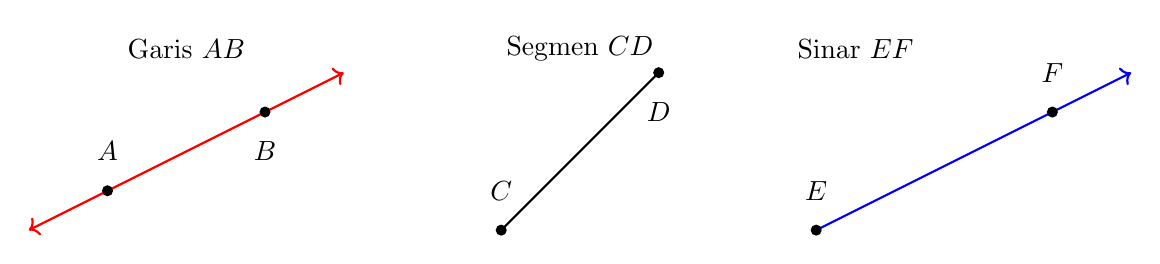
\begin{tikzpicture}
    % Draw a line
    \draw[red, thick, <->] (-4,-1) -- (0,1);
    \node at (-2,1.3) {Garis $AB$};
    \fill (-3,-0.5) circle (2pt);
    \fill (-1,0.5) circle (2pt);
    \node at (-3,-0) {$A$};
    \node at (-1,0) {$B$};

    % Draw a segment
    \draw[thick] (2,-1) -- (4,1);
    \node at (3,1.3) {Segmen $CD$};
    \fill (2,-1) circle (2pt);
    \fill (4,1) circle (2pt);
    \node at (2,-0.5) {$C$};
    \node at (4,0.5) {$D$};

    % Draw a ray
    \draw[blue, thick, ->] (6,-1) -- (10,1);
    \node at (6.5,1.3) {Sinar $EF$};
    \fill (6,-1) circle (2pt);
    \fill (9,0.5) circle (2pt);
    \node at (6,-0.5) {$E$};
    \node at (9,1) {$F$};
\end{tikzpicture}
\end{center}
\subsection{Lingkaran}

\begin{center}
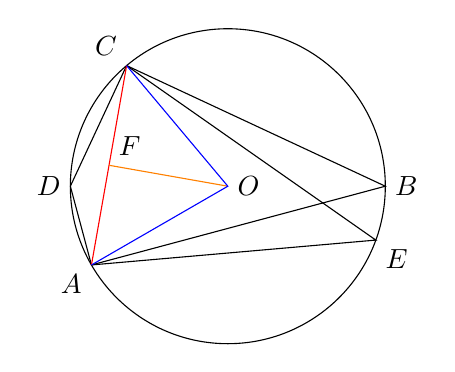
\begin{tikzpicture}
\coordinate (O) at (0,0);
\coordinate (B) at (0:2cm);
\coordinate (A) at (210:2cm);
\coordinate (D) at (180:2cm);
\coordinate (C) at (130:2cm);
\coordinate (E) at (-20:2cm);

\draw (O) circle (2cm);

\draw (A) -- (B) -- (C) -- (D) -- cycle;
\draw (A) -- (E) -- (C);
\draw[red] (A) -- (C);

\tkzDefPointBy[projection=onto A--C](O) \tkzGetPoint{F}
\draw[orange] (O) -- (F);
\draw[blue] (C) -- (O) -- (A);

\node[right] at (B) {$B$};
\node[below left] at (A) {$A$};
\node[left] at (D) {$D$};
\node[above left] at (C) {$C$};
\node[below right] at (E) {$E$};
\node[right] at (O) {$O$};
\node[above right] at (F) {$F$};
\end{tikzpicture}
\end{center}

    
Misalkan $O$ pusat lingkaran $\Gamma$ dan $A,B,C,D,E$ adalah sembarang titik pada lingkaran $\Gamma$ seperti pada gambar.
\begin{enumerate}
    \item $CO=OA$ adalah jari-jari dengan $\angle ACO = \angle OAC$.
    \item Misalkan titik $F$ adalah titik tengah tali busur $CA$, maka $OF \perp CA$ atau $OF$ tegak lurus dengan $CA$, dengan kata lain, $F$ adalah proyeksi titik $O$ ke $CA$
    \item (Sudut keliling-sudut pusat) Untuk$\angle COA = 2\angle CBA$.
    \item (sudut keliling) $\angle CBA = \angle CEA$.
    \item $ABCD$ adalah segiempat tali busur atau segiempat siklis  atau $A,B,C,D$ terletak di lingkaran (seperti pada gambar) jika dan hanya jika $\angle CBA + \angle ADC = 180^\circ$ atau $\angle ABD = \angle ACD$.
\end{enumerate}

\subsection{Latihan Soal Lingkaran}
\begin{enumerate}
    \item Pada segiempat $WXYZ$ dengan diagonal yang saling tegak lurus diketahui bahwa $\angle WZX = 30^\circ, \angle XWY = 40^\circ,$ and $\angle WYZ = 50^\circ$. Hitunglah besar $\angle X$ dan $\angle Z$.
    \begin{center}
        \includegraphics[width=0.25\textwidth]{Soal/Geometry/evanquad.PNG}
    \end{center}
		
    \item (OSK 2013) Diberikan segitiga lancip $ABC$ dengan $O$ sebagai pusat lingkaran luarnya. Misalkan $M$ dan $N$ berturut - turut pertengahan $OA$ dan $BC$. Jika $\angle ABC = 4\angle OMN$ dan $\angle ACB = 6\angle OMN$, maka besarnya $\angle OMN$ sama dengan \dots

    \item 	Pada gambar di bawah, diketahui titik A $\ne$ B pada lingkaran berdiameter $MN$ dan berpusat di $C$. $P$ adalah titik pada segmen $CN$ dimana $\angle CAP = \angle CBP = 10 ^\circ$. Jika $\angle ACM = 40^\circ$, maka $\angle BCN = \dots^\circ$	
    \begin{center}
         \includegraphics[width=0.25\textwidth]{Soal/Geometry/soalLingkaran1.PNG}
    \end{center}

    \item (OSK 2011,2012,2013,2018) Diberikan segitiga $ABC$ dan lingkaran $\Gamma$ yang berdiameter $AB$. Lingkaran $\Gamma$ memotong sisi $AC$ dan $BC$ berturut-turut di titik $D$ dan $E$. Jika $AD = \frac13 AC, BE =\frac14 BC$ dan $AB = 30$, maka luas segitiga $ABC$ adalah \dots

    \item (OSK 2015) Diberikan segitiga $ABC$ dengan sudut $\angle ABC = 90^\circ$. Lingkaran $L_1$ dengan $AB$ sebagai diameter sedangkan lingkaran $L_2$ dengan $BC$ sebagai diameternya. Kedua lingkaran $L_1$ dan $L_2$ berpotongan di $B$ dan $P$. Jika $AB = 5$, $BC = 12$ dan $BP = x$ maka nilai dari $\frac{240}{x}$ adalah \ldots
\end{enumerate}
\subsection{Lingkaran}

\begin{center}
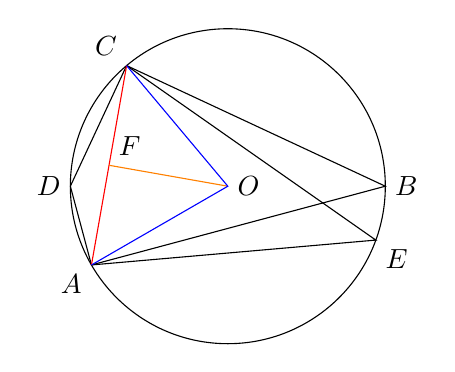
\begin{tikzpicture}
\coordinate (O) at (0,0);
\coordinate (B) at (0:2cm);
\coordinate (A) at (210:2cm);
\coordinate (D) at (180:2cm);
\coordinate (C) at (130:2cm);
\coordinate (E) at (-20:2cm);

\draw (O) circle (2cm);

\draw (A) -- (B) -- (C) -- (D) -- cycle;
\draw (A) -- (E) -- (C);
\draw[red] (A) -- (C);

\tkzDefPointBy[projection=onto A--C](O) \tkzGetPoint{F}
\draw[orange] (O) -- (F);
\draw[blue] (C) -- (O) -- (A);

\node[right] at (B) {$B$};
\node[below left] at (A) {$A$};
\node[left] at (D) {$D$};
\node[above left] at (C) {$C$};
\node[below right] at (E) {$E$};
\node[right] at (O) {$O$};
\node[above right] at (F) {$F$};
\end{tikzpicture}
\end{center}

    
Misalkan $O$ pusat lingkaran $\Gamma$ dan $A,B,C,D,E$ adalah sembarang titik pada lingkaran $\Gamma$ seperti pada gambar.
\begin{enumerate}
    \item $CO=OA$ adalah jari-jari dengan $\angle ACO = \angle OAC$.
    \item Misalkan titik $F$ adalah titik tengah tali busur $CA$, maka $OF \perp CA$ atau $OF$ tegak lurus dengan $CA$, dengan kata lain, $F$ adalah proyeksi titik $O$ ke $CA$
    \item (Sudut keliling-sudut pusat) Untuk$\angle COA = 2\angle CBA$.
    \item (sudut keliling) $\angle CBA = \angle CEA$.
    \item $ABCD$ adalah segiempat tali busur atau segiempat siklis  atau $A,B,C,D$ terletak di lingkaran (seperti pada gambar) jika dan hanya jika $\angle CBA + \angle ADC = 180^\circ$ atau $\angle ABD = \angle ACD$.
\end{enumerate}

\subsection{Latihan Soal Lingkaran}
\begin{enumerate}
    \item Pada segiempat $WXYZ$ dengan diagonal yang saling tegak lurus diketahui bahwa $\angle WZX = 30^\circ, \angle XWY = 40^\circ,$ and $\angle WYZ = 50^\circ$. Hitunglah besar $\angle X$ dan $\angle Z$.
    \begin{center}
        \includegraphics[width=0.25\textwidth]{Soal/Geometry/evanquad.PNG}
    \end{center}
		
    \item (OSK 2013) Diberikan segitiga lancip $ABC$ dengan $O$ sebagai pusat lingkaran luarnya. Misalkan $M$ dan $N$ berturut - turut pertengahan $OA$ dan $BC$. Jika $\angle ABC = 4\angle OMN$ dan $\angle ACB = 6\angle OMN$, maka besarnya $\angle OMN$ sama dengan \dots

    \item 	Pada gambar di bawah, diketahui titik A $\ne$ B pada lingkaran berdiameter $MN$ dan berpusat di $C$. $P$ adalah titik pada segmen $CN$ dimana $\angle CAP = \angle CBP = 10 ^\circ$. Jika $\angle ACM = 40^\circ$, maka $\angle BCN = \dots^\circ$	
    \begin{center}
         \includegraphics[width=0.25\textwidth]{Soal/Geometry/soalLingkaran1.PNG}
    \end{center}

    \item (OSK 2011,2012,2013,2018) Diberikan segitiga $ABC$ dan lingkaran $\Gamma$ yang berdiameter $AB$. Lingkaran $\Gamma$ memotong sisi $AC$ dan $BC$ berturut-turut di titik $D$ dan $E$. Jika $AD = \frac13 AC, BE =\frac14 BC$ dan $AB = 30$, maka luas segitiga $ABC$ adalah \dots

    \item (OSK 2015) Diberikan segitiga $ABC$ dengan sudut $\angle ABC = 90^\circ$. Lingkaran $L_1$ dengan $AB$ sebagai diameter sedangkan lingkaran $L_2$ dengan $BC$ sebagai diameternya. Kedua lingkaran $L_1$ dan $L_2$ berpotongan di $B$ dan $P$. Jika $AB = 5$, $BC = 12$ dan $BP = x$ maka nilai dari $\frac{240}{x}$ adalah \ldots
\end{enumerate}
\subsection{Segitiga}
Pada segitiga $ABC$ seperti gambar berikut:
\begin{center}
\begin{tikzpicture}
    % Define the coordinates of the vertices
    \coordinate (A) at (0,0);
    \coordinate (B) at (8,0);
    \coordinate (C) at (1.5,4);
    
    % Draw the triangle
    \draw (A) -- (B) -- (C) -- cycle;
    
    % circumcircle
    \tkzCircumCenter(A,B,C)\tkzGetPoint{O}
    \tkzDrawPoint(O)
    \tkzDrawCircle(O,A)
    
    % incircle
    \tkzDefCircle[in](A,B,C)\tkzGetPoint{I}\tkzGetLength{rIN}
    \tkzDrawPoint(I)
    \tkzDrawCircle[R](I,\rIN pt)
    
    % angle bisector
    \tkzDrawBisector[blue](B,A,C)\tkzGetPoint{E}
    \tkzDrawCircle[R](E,1 pt)
    
    %altitude
    \tkzDefPointBy[projection=onto B--C](A) \tkzGetPoint{D}
    \tkzDefPointBy[projection=onto B--A](C) \tkzGetPoint{C1}
    \tkzInterLL(A,D)(C,C1) \tkzGetPoint{H}
    \tkzDrawPoints(H) \tkzLabelPoints[below right](H)
    \tkzDrawSegment[red](A,D)
    \tkzDrawSegment[red](C,C1)

    %garis sumbu
    \tkzDefPointBy[projection=onto B--C](O) \tkzGetPoint{M}
    \tkzDefPointBy[homothety=center O ratio 3.2](M) \tkzGetPoint{M1}
    \tkzDefPointBy[homothety=center O ratio -3.2](M) \tkzGetPoint{M2}
    \tkzDrawSegment(M1,M2)
    \tkzDefPointBy[projection=onto B--A](O) \tkzGetPoint{M3}

    %centroid
    \tkzDrawSegment[green](A,M)
    \tkzDrawSegment[green](C,M3)
    \tkzInterLL(A,M)(C,M3) \tkzGetPoint{G}
    \tkzDrawPoints(G) \tkzLabelPoints[below right](G)
    
    % Label the vertices
    \node[below left] at (A) {$A$};
    \node[below right] at (B) {$B$};
    \node[above] at (C) {$C$};
    \node[below right] at (I) {$I$};
    \node[right] at (O) {$O$};
    \node[above right] at (E) {$E$};
    \node[above] at (D) {$D$};
    \node[right] at (M) {$M$};
\end{tikzpicture}
\end{center}
\begin{enumerate}
    \item Garis bagi $AE$ yaitu garis yang membagi dua sudut $A$ sama besar sehingga $\angle BAE = \angle EAC$. 
    \item Garis berat $AM$ dengan $M$ adalah titik tengah $BC$.
    \item Garis tinggi $AD$ adalah garis yang tegak lurus dengan $BC$. $D$ biasa disebut dengan proyeksi $A$ ke $BC$.
    \item Garis $OM$ adalah salah satu garis sumbu segitiga $ABC$, yaitu garis yang melewati titik tengah sisi segitiga dan tegak lurus dengan sisi itu.
    \item Pertemuan atau perpotongan ketiga garis tinggi segitiga $ABC$ adalah titik tinggi, dalam gambar ini adalah $H$ (orthocenter).
    \item Pertemuan atau perpotongan ketiga garis bagi segitiga $ABC$ adalah titik bagi atau titik pusat lingkaran dalam (incircle) segitiga $ABC$ dalam gambar ini adalah $I$ (incenter).
    \item Pertemuan atau perpotongan ketiga garis berat segitiga $ABC$ adalah titik berat (centroid).
    \item Pertemuan atau perpotongan ketiga garis sumbu segitiga $ABC$ adalah titik pusat lingkaran luar (circumcircle) segitiga $ABC$ yang dalam gambar ini adalah $O$ (circumcenter).
    \item Berlaku \textbf{ketaksamaan segitiga} yaitu $AB+BC>CA$, $BC+CA>AB$, dan $CA+AB>BC$. Selain itu juga berlaku $|AB-BC|<CA$, $|BC-CA|<AB$, dan $|CA-AB|<BC$.
\end{enumerate}
\subsection{Kesebangunan Segitiga}
\begin{center}
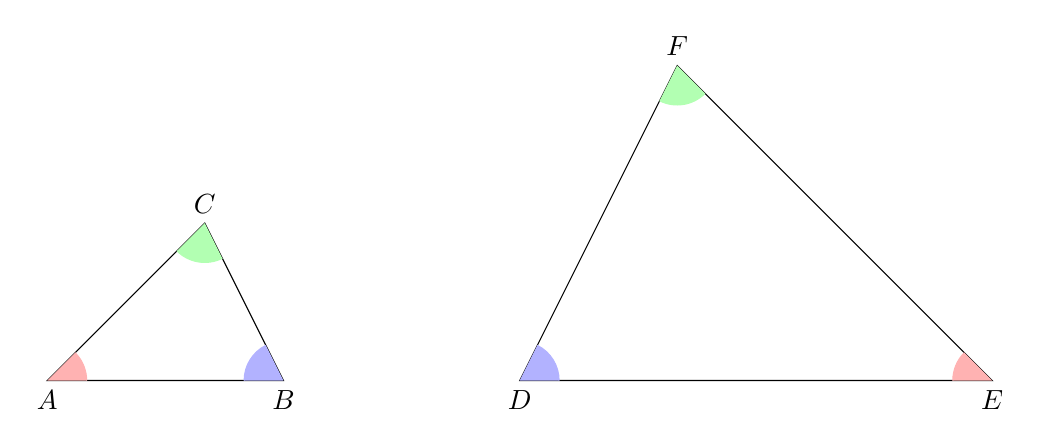
\begin{tikzpicture}
  % First triangle
  \coordinate (A) at (0,0);
  \coordinate (B) at (3,0);
  \coordinate (C) at (2,2);
  \draw (A) -- (B) -- (C) -- cycle;

  % Second triangle
  \coordinate (D) at (6,0);
  \coordinate (E) at (12,0);
  \coordinate (F) at (8,4);
  \draw (D) -- (E) -- (F) -- cycle;

  % Labeling the vertices
  \node[below] at (A) {$A$};
  \node[below] at (B) {$B$};
  \node[above] at (C) {$C$};
  \node[below] at (D) {$D$};
  \node[below] at (E) {$E$};
  \node[above] at (F) {$F$};

  \draw pic[draw=green!30,fill=green!30,angle radius=0.5cm] {angle=A--C--B};
  \draw pic[draw=green!30,fill=green!30,angle radius=0.5cm] {angle=D--F--E};
  \draw pic[draw=red!30,fill=red!30,angle radius=0.5cm] {angle=B--A--C};
  \draw pic[draw=red!30,fill=red!30,angle radius=0.5cm] {angle=F--E--D};
  \draw pic[draw=blue!30,fill=blue!30,angle radius=0.5cm] {angle=C--B--A};
  \draw pic[draw=blue!30,fill=blue!30,angle radius=0.5cm] {angle=E--D--F};
\end{tikzpicture}
\end{center}



Segitiga $ABC$ dan $DEF$ sebangun atau $ABC \sim DEF$ jika dan hanya jika minimal salah satu syarat ini terpenuhi:
\begin{enumerate}
    \item $\angle ABC = \angle DEF$ dan $\angle BAC = \angle EDF$.
    \item $\dfrac{AB}{DE} = \dfrac{BC}{EF} = \dfrac{CA}{FD}$.
    \item $\dfrac{AB}{DE} = \dfrac{BC}{EF}$ dan $\angle ABC = \angle DEF$ (sudut yang diapit dua sisi yang diperbandingkan nilainya sama)
\end{enumerate}

\subsection{Kekongruenan Segitiga}
\begin{center}
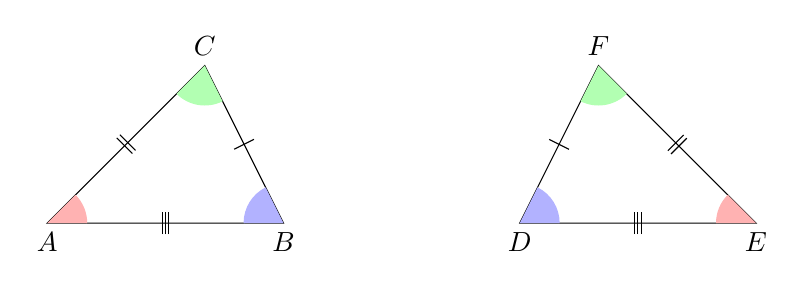
\begin{tikzpicture}
  % First triangle
  \coordinate (A) at (0,0);
  \coordinate (B) at (3,0);
  \coordinate (C) at (2,2);
  \draw (A) -- (B) -- (C) -- cycle;

  % Second triangle
  \coordinate (D) at (6,0);
  \coordinate (E) at (9,0);
  \coordinate (F) at (7,2);
  \draw (D) -- (E) -- (F) -- cycle;

  % Labeling the vertices
  \node[below] at (A) {$A$};
  \node[below] at (B) {$B$};
  \node[above] at (C) {$C$};
  \node[below] at (D) {$D$};
  \node[below] at (E) {$E$};
  \node[above] at (F) {$F$};

  \draw pic[draw=green!30,fill=green!30,angle radius=0.5cm] {angle=A--C--B};
  \draw pic[draw=green!30,fill=green!30,angle radius=0.5cm] {angle=D--F--E};
  \draw pic[draw=red!30,fill=red!30,angle radius=0.5cm] {angle=B--A--C};
  \draw pic[draw=red!30,fill=red!30,angle radius=0.5cm] {angle=F--E--D};
  \draw pic[draw=blue!30,fill=blue!30,angle radius=0.5cm] {angle=C--B--A};
  \draw pic[draw=blue!30,fill=blue!30,angle radius=0.5cm] {angle=E--D--F};

    \tkzMarkSegment[pos=.5,mark=|](C,B)
    \tkzMarkSegment[pos=.5,mark=|](D,F)
    \tkzMarkSegment[pos=.5,mark=||](C,A)
    \tkzMarkSegment[pos=.5,mark=||](E,F)
    \tkzMarkSegment[pos=.5,mark=|||](B,A)
    \tkzMarkSegment[pos=.5,mark=|||](E,D)
\end{tikzpicture}
\end{center}

Sedangkan $ABC$ dan $DEF$ dikatakan kongruen atau $\triangle ABC \cong \triangle DEF$ jika dan hanya jika $AB=DE, BC=EF, CA=FD$ atau dengan kata lain kedua segitiga tersebut sebangun dan ada salah satu sisi dari kedua segitiga tersebut yang panjangnya sama. Simpelnya kongruen = sama persis.

\input{Soal/Geometry/segitigaSebangunKongruen}


\subsection{Latihan Soal Segitiga }
\begin{enumerate}    
    \item Garis berat $AD$ pada segitiga $ABC$ memotong garis berat $CF$ di titik $P$, serta perpanjangan $BP$ memotong $AC$ di $E$. Jika diketahui segitiga $ABC$ lancip dan $AB=6$, maka panjang $DE$ adalah \dots

    \item (OSK 2011,2012,2013,2018) Diberikan segitiga $ABC$ dan lingkaran $\Gamma$ yang berdiameter $AB$. Lingkaran $\Gamma$ memotong sisi $AC$ dan $BC$ berturut-turut di titik $D$ dan $E$. Jika $AD = \frac13 AC, BE =\frac14 BC$ dan $AB = 30$, maka luas segitiga $ABC$ adalah \dots
		
    \item Diberikan segitiga $ABC$ dengan $D$ titik tengah $AC$, $E$ titik tengah $BD$, dan $H$ merupakan pencerminan $A$ terhadap $E$. Jika $F$ merupakan perpotongan antara $AH$ dengan $BC$, maka nilai $\dfrac{AF}{FH}$ sama dengan \dots
		 
    \item Diberikan segitiga $ABC$ dengan panjang sisi $BC = 20$, $CA = 24$, dan $AB=12$. Titik $D$ pada segmen $BC$ dengan $BD = 5$. Lingkaran luar dari segitiga $ABD$ memotong $CA$ di $E$. Hitunglah nilai $2 \times DE$.

    \item (OSK 2015) Diberikan trapesium $ABCD$ dengan $AB$ sejajar $DC$ dan $AB = 84$ serta $DC = 25$. Jika trapesium $ABCD$ memiliki lingkaran dalam yang menyinggung keempat sisinya, keliling trapesium $ABCD$ adalah \ldots

    \item (OSK 2022) Diberikan segitiga siku-siku $ABC$. Jika luas dari segitiga $ABC$ adalah 112. Misalkan $R$ adalah panjang jari-jari lingkaran luar segitiga $ABC$ dan $r$ adalah panjang jari-jari lingkaran dalam segitiga $ABC$. Diketahui juga $R + r = 16$. Panjang sisi miring dari segitiga $ABC$ adalah \ldots
\end{enumerate}
\subsection{Latihan Soal Segitiga }
\begin{enumerate}    
    \item Garis berat $AD$ pada segitiga $ABC$ memotong garis berat $CF$ di titik $P$, serta perpanjangan $BP$ memotong $AC$ di $E$. Jika diketahui segitiga $ABC$ lancip dan $AB=6$, maka panjang $DE$ adalah \dots

    \item (OSK 2011,2012,2013,2018) Diberikan segitiga $ABC$ dan lingkaran $\Gamma$ yang berdiameter $AB$. Lingkaran $\Gamma$ memotong sisi $AC$ dan $BC$ berturut-turut di titik $D$ dan $E$. Jika $AD = \frac13 AC, BE =\frac14 BC$ dan $AB = 30$, maka luas segitiga $ABC$ adalah \dots
		
    \item Diberikan segitiga $ABC$ dengan $D$ titik tengah $AC$, $E$ titik tengah $BD$, dan $H$ merupakan pencerminan $A$ terhadap $E$. Jika $F$ merupakan perpotongan antara $AH$ dengan $BC$, maka nilai $\dfrac{AF}{FH}$ sama dengan \dots
		 
    \item Diberikan segitiga $ABC$ dengan panjang sisi $BC = 20$, $CA = 24$, dan $AB=12$. Titik $D$ pada segmen $BC$ dengan $BD = 5$. Lingkaran luar dari segitiga $ABD$ memotong $CA$ di $E$. Hitunglah nilai $2 \times DE$.

    \item (OSK 2015) Diberikan trapesium $ABCD$ dengan $AB$ sejajar $DC$ dan $AB = 84$ serta $DC = 25$. Jika trapesium $ABCD$ memiliki lingkaran dalam yang menyinggung keempat sisinya, keliling trapesium $ABCD$ adalah \ldots

    \item (OSK 2022) Diberikan segitiga siku-siku $ABC$. Jika luas dari segitiga $ABC$ adalah 112. Misalkan $R$ adalah panjang jari-jari lingkaran luar segitiga $ABC$ dan $r$ adalah panjang jari-jari lingkaran dalam segitiga $ABC$. Diketahui juga $R + r = 16$. Panjang sisi miring dari segitiga $ABC$ adalah \ldots
\end{enumerate}

\section{Referensi}
\begin{enumerate}
\item Hermanto, Eddy. 2011. Diktat Pembinaan Olimpiade Matematika Dasar.
\end{enumerate}
	
\end{document}https://www.overleaf.com/project/61a1ae7236682644a20088dd